\documentclass[10pt]{article}
\usepackage[T1]{fontenc}
\usepackage{mathptmx}
\usepackage[paperwidth=8.5in,paperheight=11in,textwidth=6.875in,textheight=9in,top=0.9in]{geometry}
\usepackage{graphicx,float,pdfpages}
\usepackage[font=small,labelformat=empty]{caption}
\setlength{\parindent}{0pt}
\newlength{\colw}\setlength{\colw}{83.34mm}
\newcommand{\cand}[3]{\begin{figure}[H]\centering\includegraphics[width=#3]{#1}\caption{#2}\end{figure}}
\newcommand{\pair}[4]{\begin{figure}[H]\begin{minipage}[t]{\colw}\includegraphics[width=\colw]{#1}\caption{#2}\end{minipage}\hfill\begin{minipage}[t]{\colw}\includegraphics[width=\colw]{#3}\caption{#4}\end{minipage}\end{figure}}
\begin{document}
\section*{Round 3 candidates: NMI-style displays (figures at print size)}
Every figure is drawn at its final CVPR width (column 83.34 mm, text 174.6 mm) and passed the nature-figure QA (alignment, text size, collisions). Centralized, Hybrid and the capability-ladder models (GPT-5 nano, GPT-5, Gemini 3.5 Flash-Lite, Claude Sonnet 5, Qwen 3.8 Max) are still running; the scripts add them when the data land. Tables follow on the last pages.

\subsection*{Slot 1: agent scaling (number of agents)}
\cand{S1a_scaling_accuracy.pdf}{\textbf{S1a} Majority accuracy of the first $k$ agents (solid) against $k$ independent agents of the same accuracy (dashed), per data set.}{\textwidth}
\pair{S1b_neff_saturation.pdf}{\textbf{S1b} Effective number of agents saturates near 1/$\phi$; dashed, independent agents.}{S2a_gain_scatter.pdf}{\textbf{S2a} (slot 2) Multi-agent gain against SAS accuracy, marker = architecture, OLS fit.}
\cand{S1c_gain_calibration.pdf}{\textbf{S1c} Observed against predicted gain over one agent: independence (a) and beta-binomial with the observed $\phi$ (b).}{\textwidth}

\subsection*{Slot 2: capability and multi-agent gain (NMI capability ceiling)}
\cand{S2b_gain_multiples.pdf}{\textbf{S2b} Gain against SAS accuracy, one panel per architecture (Centralized and Hybrid running).}{\textwidth}

\subsection*{Slot 3: cost and accuracy (NMI economic efficiency)}
\cand{S3a_cost_fan.pdf}{\textbf{S3a} Accuracy against nominal cost per 1,000 items (log): one fan per model from SAS to each MAS; grey, Pareto frontier.}{\textwidth}
\pair{S3b_tokens_strip.pdf}{\textbf{S3b} Correct answers per 1,000 tokens by architecture; bar, geometric mean.}{S4d_debate_path.pdf}{\textbf{S4d} (slot 4) Debate trajectories: unanimity against $\phi$ from round 0 (open) to round 3 (filled).}

\subsection*{Slot 4: debate dynamics (replaces the conformity forest plot)}
\cand{S4c_debate_lines.pdf}{\textbf{S4c} Rounds 0--3 of the Decentralized MAS: $\phi$, unanimous items, majority accuracy change.}{\textwidth}

\subsection*{Slot 5: language prior (replaces the forest panels)}
\pair{S5c_prior_scatter.pdf}{\textbf{S5c} Accuracy with the blank image against the original image; diagonal, no use of the image.}{S5d_prior_slope.pdf}{\textbf{S5d} Slope chart from original to blank image per data set.}

\clearpage
\section*{Table candidates (T1a, T1b, T1b-wide, T1c, T2a, T2b)}
Generated from the results files; -- marks runs in progress. Pages follow.
\includepdf[pages=2-]{tables_preview.pdf}
\end{document}
